\documentclass[journal,compsoc]{IEEEtran}
% The preceding line is only needed to identify funding in the first footnote. If that is unneeded, please comment it out.
\usepackage[backend=biber]{biblatex}
\addbibresource{references.bib}
\usepackage{amsmath,amssymb,amsfonts}
\usepackage{algorithmic}
\usepackage{graphicx}
\usepackage{textcomp}
\usepackage{xcolor}
\usepackage{hyperref}
\usepackage{float}
\def\BibTeX{{\rm B\kern-.05em{\sc i\kern-.025em b}\kern-.08em
    T\kern-.1667em\lower.7ex\hbox{E}\kern-.125emX}}
\begin{document}

\title{Remembering and learning basic concepts of physics, signal processing and telecommunications \\
}

\maketitle

\section{Frequency}

Frequency is the number of occurrences of a repeating event per unit of time.

\[ f = \frac{1}{T} \] 

\section{Angular frequency}
In physics, angular frequency is a scalar measure of rotation rate. It refers to the angular displacement per unit time (for example, in rotation) or the rate of change of the phase of a sinusoidal waveform.
\[\omega = \frac{2\pi}{T} = 2\pi f \]

\section{Phase}
The phase of a periodic function \(F\) of some real variable \(t\) (such as time) is an angle-like quantity representing the fraction of the cycle covered up to \(t\). It is denoted \(\phi(t)\) and expressed in such a scale that it varies by one full turn as the variable \(t\) goes through each period.

The term "phase" is also used when comparing a periodic function \(F\) with a shifted version \(G\) of it. If the shift in \(t\) is expressed as a fraction of the period, and then scaled to an angle \(\varphi\) spanning a whole turn, one gets the phase shift, phase offset, or phase difference of \(G\) relative to \(F\).

\[\phi (t)=2\pi \left[\!\!\left[{\frac {t-t_{0}}{T}}\right]\!\!\right]\]

\section{Amplitude}
The amplitude of a periodic variable is a measure of its change in a single period (such as time or spatial period). There are various definitions of amplitude, which are all functions of the magnitude of the differences between the variable's extreme values. (see Fig. 1)

\begin{figure}[H]
\begin{center}
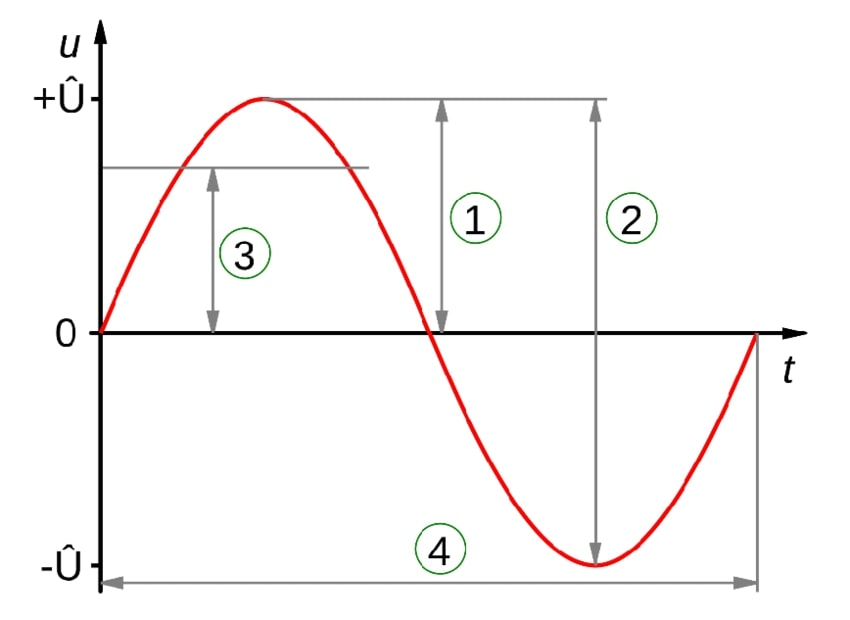
\includegraphics[scale=0.2]{amplitude}
		\caption{Peak amplitude (1), Peak-to-peak amplitude (2), Root-mean square amplitude (3), Wave period (4)}
\end{center}
\end{figure}

\section{Convolutions of signals}

A convolution is a mathematical operation applied on two functions which yields another function expressing how the shape of one is modified by the other. It is defined as the integral of the product of the two functions after one is reversed and shifted.

\[ (f * g)(t) = \int_{-\infty}^{\infty} f(\tau)g(t-\tau) \,d\tau \]

\section{Power}
In physics, power is the amount of energy transferred or converted per unit time (Joules per second).

\[ P = \frac{dW}{dt} \]

\section{Power spectrum}
The power spectrum \( S_{xx}(f)\) of a time series \(x(t)\) describes the distribution of power into frequency components composing that signal. According to Fourier analysis, any physical signal can be decomposed into a number of discrete frequencies, or a spectrum of frequencies over a continuous range. The statistical average of a certain signal or sort of signal (including noise) as analyzed in terms of its frequency content, is called its spectrum.

\section{Sound intensity}

Sound intensity, also known as acoustic intensity, is defined as the power carried by sound waves per unit area in a direction perpendicular to that area. The SI unit of intensity, which includes sound intensity, is the watt per square meter (\(W/m^2\)). One application is the noise measurement of sound intensity in the air at a listener's location as a sound energy quantity.

Sound intensity is not the same physical quantity as sound pressure. Human hearing is sensitive to sound pressure which is related to sound intensity. In consumer audio electronics, the level differences are called "intensity" differences, but sound intensity is a specifically defined quantity and cannot be sensed by a simple microphone.

Sound intensity level is a logarithmic expression of sound intensity relative to a reference intensity.

\section{Magnitude spectrum and phase spectrum}
The magnitude spectrum (referring to sound intensity) specifies the magnitude of signal components as a function of component frequency. The phase spectrum specifies the phase of signal components as a function of component frequency. 

\begin{figure}[H]
\begin{center}
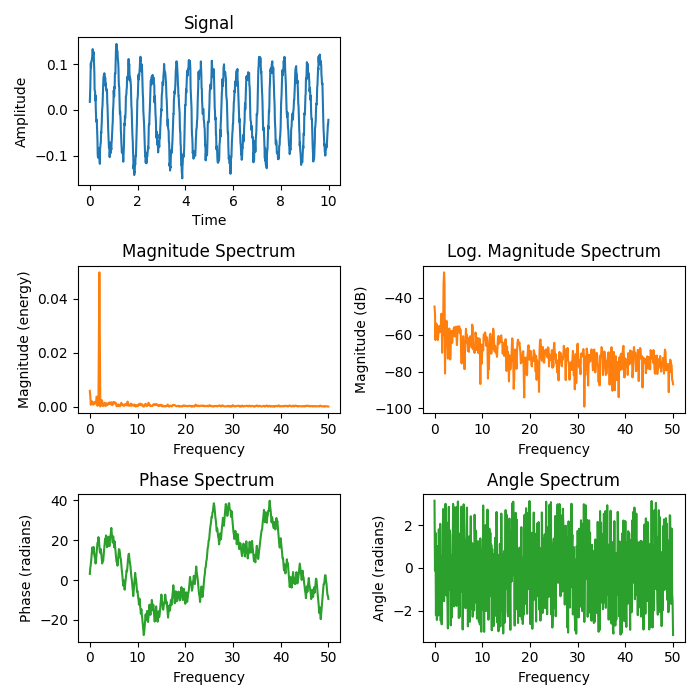
\includegraphics[scale=0.5]{magnitude_phase_spectra}
\end{center}
\end{figure}

\section{Spectrogram}
A spectrogram is a visual representation of the spectrum of frequencies of a signal as it varies with time. A spectrogram can be generated by an optical spectrometer, a bank of band-pass filters, by Fourier transform or by a wavelet transform (in which case it is also known as a scaleogram or scalogram).

\begin{figure}[H]
\begin{center}
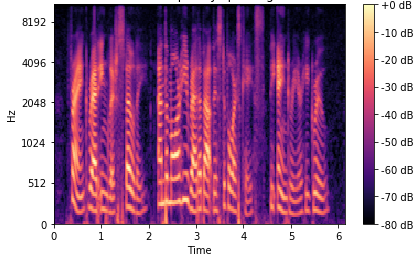
\includegraphics[scale=0.5]{spectrogram}
		\caption{Frequencies are shown increasing up the vertical axis, and time on the horizontal axis. The legend to the right shows that the color intensity increases with the sound intensity.}
\end{center}
\end{figure}

\section{Logarithmic scale}
A logarithmic scale (or log scale) is a way of displaying numerical data over a very wide range of values in a compact way - typically the largest numbers in the data are hundreds or even thousands of times larger than the smallest numbers. Such a scale is nonlinear: the numbers 10 and 20, and 60 and 70, are not the same distance apart on a log scale. Rather, the numbers 10 and 100, and 60 and 600 are equally spaced. Thus moving a unit of distance along the scale means the number has been multiplied by 10 (or some other fixed factor). Often exponential growth curves are displayed on a log scale, otherwise they would increase too quickly to fit within a small linear graph.

\section{Decibels}
The decibel is used in a wide range of applications. Decibels are especially used, when referring to power or a derived measure, whose values can vary in a wide range. The most prominent usage of decibels is in sound volume. So, for example a sound of 0dB is barely hearable, whereas a vacuum cleaner on average has 75dB and a rock concert reaches about 110dB.

When expressing a power ratio, it is defined as ten times the logarithm in base 10. That is, a change in power by a factor of 10 corresponds to a 10 dB change in level. When expressing root-power quantities, a change in amplitude by a factor of 10 corresponds to a 20 dB change in level.

Power:
\[ X_{dB} = 10\ log_{10}\left(\frac{X_{lin}}{X_{ref}}\right)\]

Amplitude:
\[ X_{dB} = 20\ log_{10}\left(\frac{X_{lin}}{X_{ref}}\right)\]

The equation transforms quantity \(X_{lin}\) from linear scale to a quantity in \(dB\) scale \(X_{dB}\). In order to do that, first the linear quantity is related to a reference quantity \(X_{ref}\) and the ratio of both powers is transformed into the log-domain. When \(X_{lin}\) is equal to the reference level, the dB-scale becomes zero.

\section{Low-pass filter}
A low-pass filter is a filter that passes signals with a frequency lower than a selected cutoff frequency and attenuates signals with frequencies higher than the cutoff frequency. The exact frequency response of the filter depends on the filter design. The filter is sometimes called a high-cut filter, or treble-cut filter in audio applications. A low-pass filter is the complement of a high-pass filter.

\section{Frequency domain}
In physics, electronics, control systems engineering, and statistics, the frequency domain refers to the analysis of mathematical functions or signals with respect to frequency, rather than time. Put simply, a time-domain graph shows how a signal changes over time, whereas a frequency-domain graph shows how much of the signal lies within each given frequency band over a range of frequencies.

\section{Frequency band}
A frequency band is an interval in the frequency domain, delimited by a lower frequency and an upper frequency. The term may refer to a radio band or an interval of some other spectrum.
Many systems are characterized by the range of frequencies to which they respond. Musical instruments produce different ranges of notes within the hearing range. The electromagnetic spectrum can be divided into many different ranges such as visible light, infrared or ultraviolet radiation, radio waves, X-rays and so on, and each of these ranges can in turn be divided into smaller ranges. A radio communications signal must occupy a range of frequencies carrying most of its energy, called its bandwidth.

\section{Filter}
In signal processing, a filter is a device or process that removes some unwanted components or features from a signal. Filtering is a class of signal processing, the defining feature of filters being the complete or partial suppression of some aspect of the signal. Most often, this means removing some frequencies or frequency bands. However, filters do not exclusively act in the frequency domain; especially in the field of image processing many other targets for filtering exist.

\section{Passband}
A passband is the range of frequencies or wavelengths that can pass through a filter. For example, a radio receiver contains a bandpass filter to select the frequency of the desired radio signal out of all the radio waves picked up by its antenna. The passband of a receiver is the range of frequencies it can receive when it is tuned into the desired frequency (channel).

A bandpass-filtered signal (that is, a signal with energy only in a passband), is known as a bandpass signal, in contrast to a baseband signal.

\section{Baseband}
In telecommunications, baseband is the range of frequencies occupied by a signal that has not been modulated to higher frequencies. Baseband signals typically originate from transducers, converting some other variable into an electrical signal. For example, the output of a microphone is a baseband signal that is an analog of the received audio. In conventional analog radio broadcasting the baseband audio signal is used, after processing, to modulate a separate RF (radio frequency) carrier signal at a much higher frequency.

\section{Narrowband}
In the audio spectrum narrowband sounds are sounds that occupy a narrow range of frequencies. In telephony, narrowband is usually considered to cover frequencies 300–3400 Hz, i.e. the voiceband.

\section{Carrier wave}
In telecommunications, a carrier wave, carrier signal, or just carrier, is a waveform (usually sinusoidal) that is modulated (modified) with an information-bearing signal for the purpose of conveying information. This carrier wave usually has a much higher frequency than the input signal does. The purpose of the carrier is usually to transmit the information through space.

\section{Modulation}
In electronics and telecommunications, modulation is the process of varying one or more properties of a periodic waveform, called the carrier signal, with a separate signal called the modulation signal that typically contains information to be transmitted. For example, the modulation signal might be an audio signal representing sound from a microphone, a video signal representing moving images from a video camera, or a digital signal representing a sequence of binary digits, a bitstream from a computer. The carrier is higher in frequency than the modulation signal. The purpose of modulation is to impress the information on the carrier wave, which is used to carry the information to another location. In radio communication the modulated carrier is transmitted through space as a radio wave to a radio receiver.

\section{Demodulation}
Demodulation is extracting the original information-bearing signal from a carrier wave. A demodulator is an electronic circuit (or computer program in a software-defined radio) that is used to recover the information content from the modulated carrier wave.

\section{Amplitude modulation}
Amplitude modulation (AM) is a modulation technique used in electronic communication, most commonly for transmitting messages with a radio wave. In amplitude modulation, the amplitude (signal strength) of the carrier wave is varied in proportion to that of the message signal, such as an audio signal. This technique contrasts with angle modulation, in which either the frequency of the carrier wave is varied, as in frequency modulation, or its phase, as in phase modulation.



\vspace{12pt}

\end{document}


